\documentclass[12pt]{article}
\usepackage{graphicx}
\usepackage{xcolor}
% \usepackage[margin=1.7cm]{geometry}
\usepackage{colortbl}
\usepackage{tikz}
\usepackage{amsmath}
\usepackage{caption}
\usepackage{subcaption}
\usepackage{textcomp}
\begin{document}
\begin{titlepage}
\begin{center}
    
\includegraphics[width=\textwidth]{./logo.png}
    \\ [2.5cm]
    \textsc{\Large Autonomous Mobile Robots}
    \\ [0.5cm]
    \textsc{\large Third assignment}
    \\ [1cm]
    \hrule
    \vspace{0.3cm}
    \textsc{Probabilistic Pose Estimation based on a Topological Map}
    \\ [0.3cm]
    \hrule
    \vfill
    \textsc{Ruben Janssen, 10252657 \\[0.2cm] David van Erkelens, 10264019 \\[0.7cm] Department of Computer Science \\ University of Amsterdam \\[0.3cm] \today}
\end{center}
\end{titlepage}
\tableofcontents
\clearpage
\section{Introduction}
In order for an autonomous mobile robot to drive and navigate, it requires some method by which to determine its position. This is called the localization problem. One of the methods to solve this problem is by using probabilistic pose estimation based on a topological map. The robot tries to estimate its position with respect to known locations in the environment. This can be achieved by comparing its current position to known locations and estimating which locations is most similar. The most similar location is probably the current location of the robot.

\section{Setup}
In order to compare the robots current position with that of known locations, the robot is provided a training set of pictures. These pictures are made in different positions in the training area by using an omnidirectional camera. Based on lines and blobs detected in the pictures, the robot can compare the lines and blobs detected in the picture taken at the current position to the provided pictures. Unfortunately however, not enough robots were available to test with. Instead, the software compares the known locations to a set of given photos rather than to a live video feed.

\clearpage

\section{Implementation}
\subsection{Detecting Lines}
Before pictures can be compared, they have to be analysed. First, the walls are detected around the robot (figure \ref{fig:points}). Second, the detected walls are mapped on a grid corresponding with their distance from the vehicle (figure \ref{fig:grid}). Third, the lines are extracted from the grid (figure \ref{fig:lines}).
\begin{figure}[h!]
	\centering
	\begin{subfigure}[b]{0.3\textwidth}
            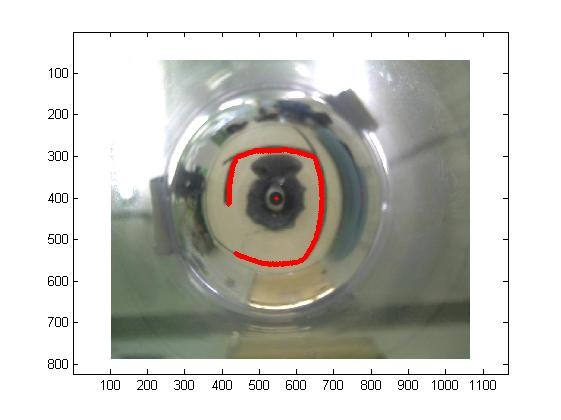
\includegraphics[width=\textwidth]{points.jpg}
            \caption{Detecting walls}
            \label{fig:points}
    \end{subfigure}
    ~
    \begin{subfigure}[b]{0.3\textwidth}
            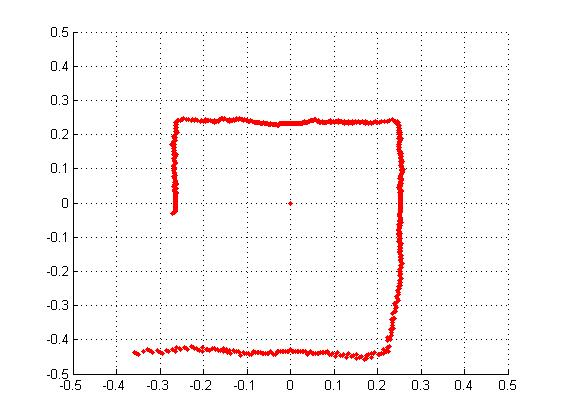
\includegraphics[width=\textwidth]{grid.jpg}
            \caption{Distance grid}
            \label{fig:grid}
    \end{subfigure}
    ~
    \begin{subfigure}[b]{0.3\textwidth}
            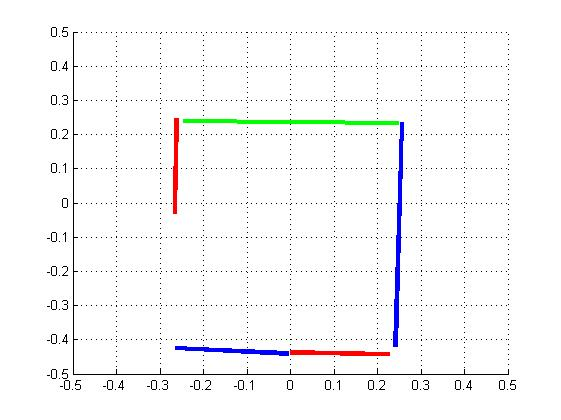
\includegraphics[width=\textwidth]{lines.jpg}
            \caption{Forming lines}
            \label{fig:lines}
    \end{subfigure}
    \caption{Detecting lines}
\end{figure}
pints, grid, lines.jpg

The code to determine points and calculate the distance grid are provided. To extract the lines from the distance grid, a simpified version of the Split \& Merge algorithm is used. 

GetLinePattern.m
 
\subsection{Comparing Lines}
lineschance.jpg
checkLinePattern.m

\subsection{Detecting Blobs}
blobs.jpg
GetBlobPattern.m

\subsection{Comparing Blobs}
blobschance.jpg
checkBlobPattern.m

\subsection{Combining Blobs and Lines}
% weight_average.m
% fuse_sigs.m
% lines_and_blobs_chance_fusion.jpg
% lines_and_blobs_chance_weighted.jpg
\section{Conclusion}
dd

\end {document}